\documentclass[11pt,twoside,a4paper]{article}
% http://www-h.eng.cam.ac.uk/help/tpl/textprocessing/latex_maths+pix/node6.html symboles de math
% http://fr.wikibooks.org/wiki/Programmation_LaTeX Programmation latex (wikibook)
%=========================== En-Tete =================================
%--- Insertion de paquetages (optionnel) ---
\usepackage[french]{babel}   % pour dire que le texte est en fran{\'e}ais
\usepackage{a4}	             % pour la taille   
\usepackage[T1]{fontenc}     % pour les font postscript
\usepackage{epsfig}          % pour gerer les images
%\usepackage{psfig}
\usepackage{amsmath, amsthm} % tres bon mode mathematique
\usepackage{amsfonts,amssymb}% permet la definition des ensembles
\usepackage{float}           % pour le placement des figure
\usepackage{verbatim}

\usepackage{longtable} % pour les tableaux de plusieurs pages

\usepackage[table]{xcolor} % couleur de fond des cellules de tableaux

\usepackage{lastpage}

\usepackage{multirow}

\usepackage{multicol} % pour {\'e}crire dans certaines zones en colonnes : \begin{multicols}{nb colonnes}...\end{multicols} 

% \usepackage[top=1.5cm, bottom=1.5cm, left=1.5cm, right=1.5cm]{geometry}
% gauche, haut, droite, bas, entete, ente2txt, pied, txt2pied
\usepackage{vmargin}
\setmarginsrb{0.20cm}{0.20cm}{0.20cm}{0.20cm}{15pt}{3pt}{15pt}{3pt}

\usepackage{lscape} % changement orientation page
%\usepackage{frbib} % enlever pour obtenir references en anglais
% --- style de page (pour les en-tete) ---
\pagestyle{empty}

% % % en-tete et pieds de page configurables : fancyhdr.sty

% http://www.trustonme.net/didactels/250.html

% http://ww3.ac-poitiers.fr/math/tex/pratique/entete/entete.htm
% http://www.ctan.org/tex-archive/macros/latex/contrib/fancyhdr/fancyhdr.pdf
% \usepackage{fancyhdr}
% \pagestyle{fancy}
% % \newcommand{\chaptermark}[1]{\markboth{#1}{}}
% % \newcommand{\sectionmark}[1]{\markright{\thesection\ #1}}
% \fancyhf{}
% \fancyhead[LE,RO]{\bfseries\thepage}
% \fancyhead[LO]{\bfseries\rightmark}
% \fancyhead[RE]{\bfseries\leftmark}
% \fancyfoot[LE]{\thepage /\pageref{LastPage} \hfill
	% TITLE
% \hfill 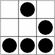
\includegraphics[width=0.5cm]{img/logo_glider.png} }
% \fancyfoot[RO]{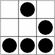
\includegraphics[width=0.5cm]{img/logo_glider.png} \hfill
	% TITLE
% \hfill \thepage /\pageref{LastPage}}
% \renewcommand{\headrulewidth}{0.5pt}
% \renewcommand{\footrulewidth}{0.5pt}
% \addtolength{\headheight}{0.5pt}
% \fancypagestyle{plain}{
	% \fancyhead{}
	% \renewcommand{\headrulewidth}{0pt}
% }


%============================= Corps =================================
\begin{document}

\setlength\parindent{0pt}

\texttt{http://rue89.nouvelobs.com/2015/01/23/syndrome-truman-show-257280}~\\

\textbf{\LARGE Le syndrome Truman Show} ~\\

\emph{\small par Mike Jay, journaliste, le 23/01/2015 {\`a} 13h05 --- ULYCES } ~\\

\begin{minipage}[ht]{7.00cm}
	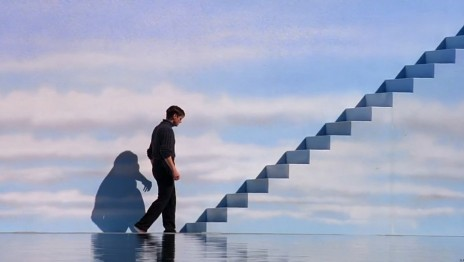
\includegraphics[width=6.95cm]{img/1353349429-screen-shot-2011-03-29-at-5-09-52-pm-2.jpg}~\\
	\emph{\footnotesize Truman Burbank (Jim Carrey) dans <<The Truman Show>> de Peter Weir (1998) }
\end{minipage} \hfill \begin{minipage}[ht]{0.65\textwidth}
	Les articles de psychiatrie clinique connaissent la plupart du temps un retentissement assez limit{\'e} dans les m{\'e}dias g{\'e}n{\'e}ralistes. Il appara{\^i}t pourtant justifi{\'e} qu'un papier [\texttt{PDF~\footnotemark}] intitul{\'e} <<The Truman Show Delusion : Psychosis in the Global Village>> (en fran\c{c}ais : <<Le syndrome Truman Show : psychose dans le \texttt{village global~\footnotemark}>>) ait lui-m{\^e}me suscit{\'e} un int{\'e}r{\^e}t global. ~\\

	Ses auteurs, les fr{\`e}res Joel et Ian Gold, y pr{\'e}sentaient une s{\'e}rie frappante de cas cliniques : des individus ayant la conviction qu'ils {\'e}taient secr{\`e}tement film{\'e}s pour une {\'e}mission de t{\'e}l{\'e}r{\'e}alit{\'e}.~\\
\end{minipage}~\\~\\
\footnotetext[1]{\texttt{http://ts-si.org/files/doi101080135468052012666113.pdf}}
\footnotetext{\texttt{http://fr.wikipedia.org/wiki/Village\_planetaire}}

Dans un de ces cas, le sujet s'est rendu {\`a} New York et a exig{\'e} de rencontrer le <<r{\'e}alisateur>> du film de sa vie. Il souhaitait {\'e}galement v{\'e}rifier si le World Trade Center avait r{\'e}ellement {\'e}t{\'e} d{\'e}truit, ou si cela s'{\'e}tait uniquement produit dans le film qu'on tournait en son honneur.~\\

Autre cas : un journaliste hospitalis{\'e} durant un {\'e}pisode maniaque s'est persuad{\'e} que ce sc{\'e}nario m{\'e}dical {\'e}tait une mise en sc{\`e}ne, et qu'il recevrait un prix pour avoir couvert les {\'e}v{\'e}nements une fois la v{\'e}rit{\'e} r{\'e}v{\'e}l{\'e}e... ~\\

Un autre sujet, lui, travaillait effectivement sur une {\'e}mission de t{\'e}l{\'e}r{\'e}alit{\'e}, et il en est venu {\`a} croire que ses coll{\`e}gues de l'{\'e}quipe de tournage le filmaient en secret. Il guettait ainsi sans cesse le moment o{\`u} les cam{\'e}ras se tourneraient vers lui et o{\`u} il se r{\'e}v{\'e}lerait {\^e}tre la v{\'e}ritable star de l'{\'e}mission. ~\\

\begin{minipage}[ht]{0.65\textwidth}
	\textbf{\Large Exemples extr{\^e}mes d'un malaise r{\'e}pandu}~\\
	
	Peu d'{\'e}ditorialistes ont {\'e}t{\'e} capables de r{\'e}sister {\`a} l'id{\'e}e que ces cas -- tous diagnostiqu{\'e}s comme schizophr{\`e}nes ou bipolaires et mis sous traitement antipsychotique -- repr{\'e}sentaient en quelque sorte la partie {\'e}merg{\'e}e de l'iceberg, r{\'e}v{\'e}lateurs d'une pathologie touchant notre culture toute enti{\`e}re.~\\
	
	On a fait d'eux les exemples extr{\^e}mes d'un malaise moderne tr{\`e}s r{\'e}pandu : une obsession de la c{\'e}l{\'e}brit{\'e} qui fait de nous les vedettes narcissiques de nos propres vies, les victimes d'une culture satur{\'e}e d'images qui d{\'e}forme notre conception de la r{\'e}alit{\'e} et brouille la fronti{\`e}re entre le r{\'e}el et l'imaginaire.~\\
	
	Ces cas semblaient parfaitement illustrer l'air du temps, tels des contes dont la morale viserait une {\'e}poque o{\`u} notre exp{\'e}rience de la r{\'e}alit{\'e} est morcel{\'e}e, et personnalis{\'e}e de fa\c{c}on insidieuse. Une {\'e}poque o{\`u} tout, de notre courrier ind{\'e}sirable {\`a} nos recherches sur Internet, contribue discr{\`e}tement {\`a} nous persuader que nous sommes le centre de l'univers.~\\
	
	Mais si le syndrome Truman Show para{\^i}t aussi {\'e}trangement en harmonie avec notre {\'e}poque, c'est en partie parce que les blockbusters hollywoodiens reposent d{\'e}sormais fr{\'e}quemment sur des r{\'e}cits qui, jusqu'{\`a} r{\'e}cemment, {\'e}taient encore confin{\'e}s aux dossiers des patients et {\`a} la litt{\'e}rature clinique sur la psychose parano{\"i}aque.~\\
\end{minipage} \hfill \begin{minipage}[ht]{0.33\textwidth}
	\small
	\hrule
	\textbf{\large Making of}~\\
	
	L'int{\'e}gralit{\'e} de cette histoire vraie sign{\'e}e Mike Jay, in{\'e}dite en fran\c{c}ais, est disponible sur Ulyces. Cette maison d'{\'e}dition num{\'e}rique publie chaque jour des histoires vraies s{\'e}lectionn{\'e}es pour leur qualit{\'e} litt{\'e}raire et leur exigence journalistique (vous pouvez les acheter {\`a} l'unit{\'e} ou vous abonner).~\\
	
	<<Le syndrome Truman Show>> est une histoire traduite de l'anglais par Cl{\'e}ment Martin d'apr{\`e}s l'article <<The Reality Show>>, paru dans Aeon en ao{\^u}t 2013. Si vous aimez les histoires li{\'e}es {\`a} la m{\'e}decine, d{\'e}couvrez sur Ulyces \texttt{<<Un monde sans antibiotique>>~\footnote{\texttt{http://www.ulyces.co/maryn-mckenna/a-quoi-ressemblera-un-monde-sans-antibiotique/}}}, \texttt{<<Docteur Hamlin en Ethiopie>>~\footnote{\texttt{http://www.ulyces.co/vincent-defait/docteur-hamlin-en-ethiopie-hopital/}}} ou encore, \texttt{<<S'enfuir du labyrinthe>>~\footnote{\texttt{http://www.ulyces.co/michael-regnier/maladie-alzheimer/}}}.~\\ 
	
	\textbf{Rue89}~\\
	\hrule
\end{minipage}~\\

La culture populaire regorge d'histoires dans lesquelles la technologie sert {\`a} observer et contr{\^o}ler secr{\`e}tement nos pens{\'e}es, ou dans lesquelles la r{\'e}alit{\'e} est simul{\'e}e {\`a} l'aide de constructions virtuelles ou de souvenirs implant{\'e}s. On ne peut y entrapercevoir la v{\'e}rit{\'e} que durant des s{\'e}quences de r{\^e}ve d{\'e}form{\'e}es, ou lors des rares occasions o{\`u} le masque tombe enfin.~\\

\textbf{\Large Le concept des <<machines {\`a} influencer>>}~\\

Quelques dizaines d'ann{\'e}es plus t{\^o}t, de telles inclinations, dans la fiction, caract{\'e}risaient les personnages fous, voire, bien souvent, les meurtriers psychotiques. De nos jours, ces m{\^e}mes traits qualifieront plus volontiers un personnage qui, comme le Truman Burbank incarn{\'e} par Jim Carrey, a r{\'e}ellement d{\'e}couvert une machination soigneusement orchestr{\'e}e, dissimul{\'e}e aux yeux de ceux qui l'entourent.~\\

Ces histoires font bien s{\^u}r {\'e}cho {\`a} notre modernit{\'e} satur{\'e}e de technologie. Ce qui est moins clair, c'est la raison pour laquelle elles adoptent une perspective qui {\'e}tait jusque-l{\`a} caract{\'e}ristique d'une rupture radicale avec la r{\'e}alit{\'e}. Cela sugg{\`e}re-t-il que les technologies m{\'e}diatiques nous rendent tous parano{\"i}aques ? Ou bien que les d{\'e}lires parano{\"i}aques sont subitement devenus plus compr{\'e}hensibles qu'ils ne l'{\'e}taient par le pass{\'e} ?~\\ 

\begin{minipage}[ht]{0.65\textwidth}
	La premi{\`e}re personne {\`a} avoir examin{\'e} cette curieuse symbiose entre nouvelles technologies et sympt{\^o}mes psychotiques est Victor Tausk, un des premiers disciples de Sigmund Freud. En 1919, il publia un article sur un ph{\'e}nom{\`e}ne qu'il appelait la <<machine {\`a} influencer>>.~\\

	Tausk avait remarqu{\'e} que les patients schizophr{\`e}nes (un diagnostic r{\'e}cemment invent{\'e}) {\'e}taient souvent convaincus que leur esprit et leur corps {\'e}taient contr{\^o}l{\'e}s par des technologies avanc{\'e}es et visibles d'eux seuls. Ces <<machines {\`a} influencer>> {\'e}taient souvent d'une conception tr{\`e}s {\'e}labor{\'e}e et model{\'e}es d'apr{\`e}s les nouveaux appareils qui transformaient la vie moderne d'alors.~\\
	
	Des patients racontaient qu'ils recevaient des messages transmis par des batteries, des bobines et autres dispositifs {\'e}lectriques cach{\'e}s. Les voix dans leur t{\^e}te {\'e}taient transmises par des formes avanc{\'e}es de t{\'e}l{\'e}phone ou de phonographe, tandis que des hallucinations visuelles r{\'e}sultaient de l'action secr{\`e}te d'une <<lanterne magique ou du cin{\'e}matographe>>. L'{\'e}tude de cas la plus d{\'e}taill{\'e}e que Tausk a men{\'e}e {\`a} bien portait sur une patiente nomm{\'e}e <<Natalija A.>>, qui croyait ses pens{\'e}es contr{\^o}l{\'e}es et son corps manipul{\'e} par un dispositif {\'e}lectrique actionn{\'e} secr{\`e}tement par des docteurs {\`a} Berlin. L'appareil avait la forme de son corps, mais le ventre {\'e}tait un couvercle doubl{\'e} de velours qui pouvait {\^e}tre ouvert et r{\'e}v{\'e}lait alors des batteries correspondant {\`a} ses organes internes.~\\
\end{minipage} \hfill \begin{minipage}[ht]{7.00cm}
	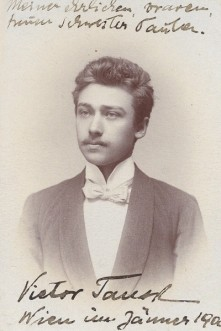
\includegraphics[width=6.95cm]{img/ulyces-trumanshow-03.jpg}~\\
	\emph{\footnotesize Victor Tausk (Wikimedia Commons/CC) }
\end{minipage}~\\
%% \footnotetext{\texttt{http://fr.wikipedia.org/wiki/Victor_Tausk#mediaviewer/File:Viktor_Tausk_%281900%...}}

\textbf{\Large De nouveaux mots pour d{\'e}crire un mal}~\\

Bien que de telles convictions fussent compl{\`e}tement d{\'e}lirantes, Tausk d{\'e}cela une certaine logique dans leur folie : comme un reflet des r{\^e}ves et des cauchemars d'un monde en proie {\`a} une {\'e}volution rapide. Les dynamos {\'e}lectriques inondaient les villes europ{\'e}ennes d'{\'e}lectricit{\'e} et de lumi{\`e}re, et les ramifications de ces r{\'e}seaux faisaient {\'e}cho aux structures en filigrane qu'on d{\'e}couvrait en laboratoire sur des lames de microscope, qui levaient le voile sur le syst{\`e}me nerveux humain.~\\

Des d{\'e}couvertes r{\'e}centes, comme les rayons X et la radio, r{\'e}v{\'e}laient des mondes jusque-l{\`a} invisibles et l'existence de myst{\'e}rieuses {\'e}nergies, qui faisaient l'objet de discussions quotidiennes dans les journaux de vulgarisation scientifique, d'extrapolations dans les \texttt{pulps~\footnote{\texttt{http://fr.wikipedia.org/wiki/Pulp\_(magazine)}}}, et qui {\'e}taient d'apr{\`e}s les spiritualistes la preuve de l'existence d'un <<au-del{\`a}>>. --- Mais pour Tausk, ces innovations ne cr{\'e}aient pas de nouvelles formes de maladie mentale. Ces d{\'e}veloppements modernes fournissaient aux patients de nouveaux mots pour d{\'e}crire leur mal.~\\

D'apr{\`e}s lui, on trouvait au c\oe ur de la schizophr{\'e}nie une <<perte des limites de l'ego>> qui rendait les sujets incapables d'imposer leur volont{\'e} sur la r{\'e}alit{\'e}, ou de se forger une id{\'e}e coh{\'e}rente de leur moi. D{\'e}pourvus qu'ils {\'e}taient de volont{\'e} propre, il leur semblait que les pens{\'e}es et les mots d'autres personnes {\'e}taient introduits de force dans leur t{\^e}te et {\'e}mis par leur bouche, alors que leur corps {\'e}tait manipul{\'e} comme celui d'une poup{\'e}e, soumis {\`a} la torture ou bien install{\'e} dans de myst{\'e}rieuses positions.~\\

Ces sensations n'avaient aucune explication rationnelle, mais ceux qui les {\'e}prouvaient {\'e}taient n{\'e}anmoins sujets {\`a} ce que Tausk appelait <<le besoin de causalit{\'e} inh{\'e}rent {\`a} l'homme>>. Ils se sentaient {\`a} la merci de forces ext{\'e}rieures n{\'e}fastes, et leur inconscient fabriquait une explication avec ce qu'il avait sous la main, d'une fa\c{c}on souvent frappante de na{\"i}vet{\'e}. Incapables de donner un sens au monde, ils se faisaient le r{\'e}ceptacle des artefacts culturels et des suppositions qui les entouraient.~\\

Quand vint le d{\'e}but du XXe si{\`e}cle, nombre d'entre eux acquirent la conviction in{\'e}branlable qu'un op{\'e}rateur cach{\'e} les tourmentait {\`a} l'aide d'une technologie avanc{\'e}e. --- La th{\'e}orie de Tausk {\'e}tait radicale en ce qu'elle impliquait que les propos d'un psychotique n'{\'e}taient pas un charabia al{\'e}atoire mais plut{\^o}t un assemblage, souvent habilement construit, de croyances et de pr{\'e}occupations collectives. --- Jusqu'alors, {\`a} travers l'histoire, le cadre explicatif pour de telles exp{\'e}riences {\'e}tait essentiellement religieux : on y voyait une possession par un esprit mal{\'e}fique, une visite du divin, de la sorcellerie, ou m{\^e}me l'emprise du d{\'e}mon. A l'{\'e}poque moderne, ces croyances restaient fr{\'e}quentes, mais des explications alternatives {\'e}taient d{\'e}sormais {\`a} port{\'e}e de main.~\\

\textbf{\Large Implants magn{\'e}tiques dans le cerveau}~\\

Tausk observa que les hallucinations dont les patients psychotiques faisaient l'exp{\'e}rience {\'e}taient typiquement non pas des objets tridimensionnels, mais des projections <<vues sur un seul plan, sur les murs ou les carreaux d'une fen{\^e}tre>>. --- La technologie nouvelle du cin{\'e}ma reproduisait pr{\'e}cis{\'e}ment cette sensation et en repr{\'e}sentait par bien des aspects une explication rationnelle : une explication qui <<ne d{\'e}montre aucune erreur de jugement, au-del{\`a} du fait de son inexistence>>.~\\

Par leur appr{\'e}hension instinctive des pouvoirs et des menaces implicites de la technologie, les machines {\`a} influencer peuvent d{\'e}montrer un aspect futuriste convaincant, voire une prescience {\'e}tonnante. Le tout premier cas attest{\'e}, datant de 1810, {\'e}tait un patient de l'h{\^o}pital psychiatrique de Bedlam appel{\'e} James Tilly Matthews, qui r{\'e}alisa de magnifiques dessins techniques de la machine qui contr{\^o}lait son esprit. --- La <<machine pneumatique>>, comme il l'appelait, utilisait les derni{\`e}res avanc{\'e}es de la science -- gaz artificiels et \texttt{magn{\'e}tisme mesm{\'e}rien~\footnote{\texttt{http://www.ampere.cnrs.fr/parcourspedagogique/zoom/mythesetlegendes/mesmerisme/}}} -- afin de conduire des courants invisibles jusqu'{\`a} son cerveau, dans lequel un aimant avait {\'e}t{\'e} implant{\'e} pour les recevoir. Le monde de rayons et de courants charg{\'e}s {\'e}lectriquement imagin{\'e} par Matthews, bien que pure folie pour ses contemporains, fait d{\'e}sormais partie int{\'e}grante de notre culture.~\\

Une rapide recherche sur Internet r{\'e}v{\`e}le que des dizaines de communaut{\'e}s en ligne se consacrent {\`a} des discussions sans fin sur les implants magn{\'e}tiques c{\'e}r{\'e}braux, r{\'e}els ou imaginaires. --- L'interpr{\'e}tation du syndrome Truman Show donn{\'e}e par les fr{\`e}res Gold suit une logique similaire. On pourrait croire {\`a} un ph{\'e}nom{\`e}ne nouveau ayant {\'e}merg{\'e} en r{\'e}ponse {\`a} notre culture m{\'e}diatique hyper-moderne, mais il s'agit en fait d'une maladie bien connue, qui a subi une cure de jouvence. Les fr{\`e}res Gold font une distinction fondamentale entre :
\begin{itemize}
    \item[$\bullet$] le \textbf{contenu des d{\'e}lires}, spectaculairement vari{\'e} et imaginatif ;
    \item[$\bullet$] et les \textbf{formes basiques} de ces derniers, qu'ils d{\'e}crivent {\`a} la fois comme <<universelles et relativement peu nombreuses>>.
\end{itemize} %% ~\\

Les d{\'e}lires de pers{\'e}cution, par exemple, se retrouvent {\`a} travers l'histoire et dans diff{\'e}rentes cultures. Un nomade vivant dans le d{\'e}sert aura plus de chances de croire qu'il est enterr{\'e} vivant dans le sable par un djinn, et un citadin Am{\'e}ricain qu'on lui a implant{\'e} une puce {\'e}lectronique et que la CIA le surveille. <<Pour une maladie souvent d{\'e}crite comme une rupture avec la r{\'e}alit{\'e}>>, observent les fr{\`e}res Gold, <<la psychose se tient remarquablement bien au fait de la r{\'e}alit{\'e}.>>~\\

\textbf{\Large D{\'e}vor{\'e}s par la culture qui les entoure}~\\

Plut{\^o}t que d{\'e}tach{\'e}s de la culture qui les entoure, les sujets psychotiques peuvent {\^e}tre vus comme d{\'e}vor{\'e}s par cette derni{\`e}re : incapables d'{\'e}tablir les limites du moi, ils sont {\`a} la merci de leur sensibilit{\'e} aigu{\"e} {\`a} l'environnement mena\c{c}ant qui les entoure. --- Si l'on s'en remet {\`a} cette interpr{\'e}tation, le syndrome Truman Show est l'expression contemporaine d'une forme commune de psychose : le d{\'e}lire grandiose. --- Les victimes des premi{\`e}res manifestations de la psychose ont souvent la conviction que le monde a connu un changement subtil, qui les place d{\'e}sormais sur le devant d'une sc{\`e}ne aux dimensions universelles. Tout est soudain riche de sens, chaque minuscule d{\'e}tail est charg{\'e} de significations personnelles. Les gens qui vous entourent sont souvent complices : ils jouent des r{\^o}les assign{\'e}s au pr{\'e}alable et vous mettent {\`a} l'{\'e}preuve ou vous pr{\'e}parent pour le moment imminent de la r{\'e}v{\'e}lation.~\\

De telles exp{\'e}riences ont jadis {\'e}t{\'e} interpr{\'e}t{\'e}es comme une visite c{\'e}leste, une transformation magique, ou comme une initiation {\`a} une r{\'e}alit{\'e} sup{\'e}rieure. On imagine ais{\'e}ment comment, si aujourd'hui elles s'imposaient subitement {\`a} nous, nous arriverions imm{\'e}diatement {\`a} la conclusion que l'explication r{\'e}side dans un quelconque complot de la t{\'e}l{\'e}vision ou des r{\'e}seaux sociaux. Ou bien que, pour une raison d{\'e}lib{\'e}r{\'e}ment gard{\'e}e secr{\`e}te, l'attention du monde serait soudainement centr{\'e}e sur nous, et qu'un public invisible nous observerait, fascin{\'e}, attendant de voir quelle serait notre r{\'e}action.~\\

Ainsi, le syndrome Truman Show n'implique pas n{\'e}cessairement que la t{\'e}l{\'e}r{\'e}alit{\'e} est une cause ou un sympt{\^o}me de maladie mentale. Il se pourrait simplement que l'omnipr{\'e}sence de la t{\'e}l{\'e}r{\'e}alit{\'e} dans notre culture offre une explication plausible {\`a} des sensations et des {\'e}v{\'e}nements inexplicables autrement.~\\

\end{document}
